\section{Muhammad Reza Syachrani - 1174084}
\subsection{Teori}
\begin{enumerate}
	\item Jelaskan apa itu klasifikasi teks, dan gambar ilustrasi
	\hfill\\
klasifikasi teks adalah cara untuk mengklasifikasikan atau mengelompokkan teks berdasarkan parameter tertentu baik itu jenis teks atau jenis dari dokumen yang terdapat kumpulan teks didalamnya. 
\begin{figure}[H]
    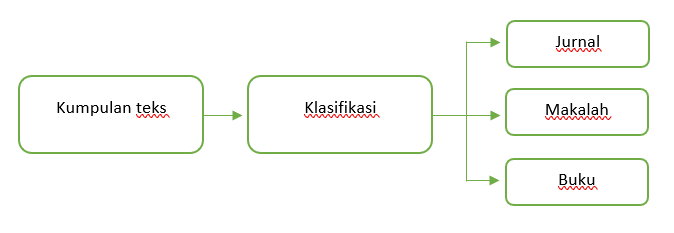
\includegraphics[width=12cm]{figures/1174084/4/teori1.png}
    \centering
    \caption{contoh klasifikasi teks}
\end{figure}

\item Jelaskan mengapa klasifikasi pada bunga tidak bisa menggunakan machine learning, sertakan ilustrasi.
	\hfill\\
	karna melakukan klasifikasi pada bunga tidak dapat menggunakan mesin learning karena terdapat banyak jenis-jenis bunga yang mirip hingga ada yang sama persis tetapi tidak sama. oleh karena itu klasifikasi bunga tida bisa dilakukan oleh mesin learning dikarenakan jika inputan ciri-ciri tidak sesuai maka bunga di inputkan kemungkinan jawaban dari mesin learning itu tidak tepat contoh menginpukan ciri-ciri bunga seroja tetapi pada mesin learning menjawab itu merupakan ciri-ciri bunga teratai.

\begin{figure}[H]
    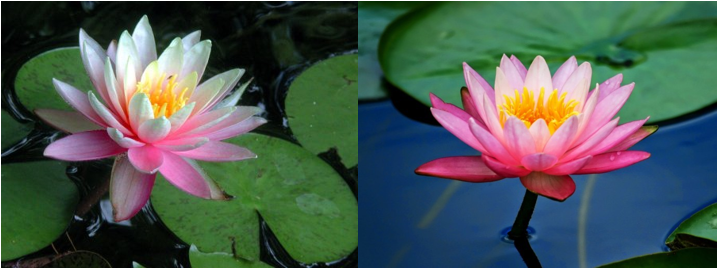
\includegraphics[width=12cm]{figures/1174084/4/teori2.png}
    \centering
    \caption{contoh klasifikasi bunga}
\end{figure}

\item Jelaskan bagaimana teknik pembelajaran mesin pada teks pada kata-kata yang digunakan di youtube.
	\hfill\\
	cara pembelajaran teks yang digunakan pada youtube yaitu dengan cara menyimpan inputan data teks pada menu pencarian youtube. sehingga pada saat kita akan mencari data yang serupa maka youtube menyediakan rekomendasi-rekomendasi dari pencaharian. contoh pada menu pencarian kita menulis kata sa maka akan muncul banyak rekomendasi yang serupa yang sering di cari oleh orang dalam jangka waktu tertentu.
\begin{figure}[H]
    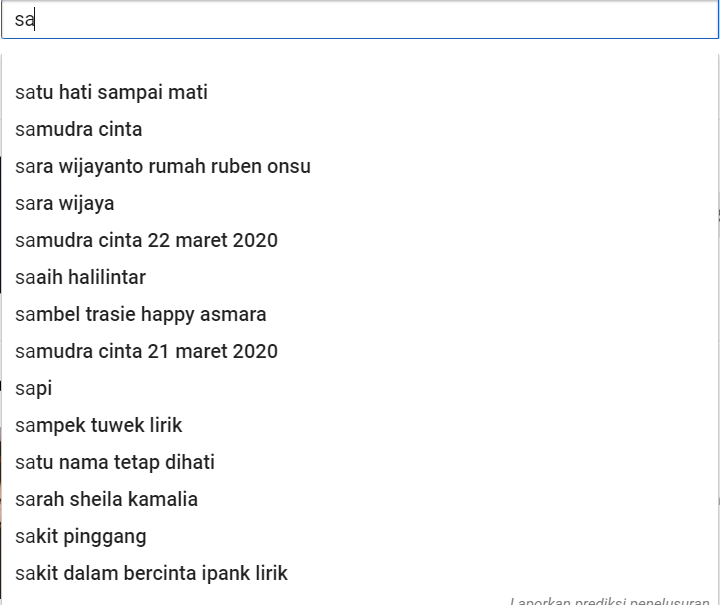
\includegraphics[width=12cm]{figures/1174084/4/teori3.png}
    \centering
    \caption{contoh teknik pembelajaran mesin}
\end{figure}

\item Jelaskan apa yang dimaksud vektorisasi data
\hfill\\
	vektorisasi data merupakan pembagian data menjadi bagian-bagian yang lebih sederhana, contoh pada satu paragraf terdiri dari 200 kata kemudian dilakukan vektorisasi dengancara membagi-bagi kata dalam paragraf tersebut ke dalam kalimat-kalimat yang terpisah kemudian di pecah lagi menjadi data dalam perkata selanjutnya kata kata tersebut di terjemahkan.	

\item Jelaskan apa itu bag of words dan ilustrasi
	\hfill\\
bag of words merupakan representasi teks yang menggambarkan kemunculan kata-kata dalam dokumen. ePngelompokan kata kata kedalam perhitunga, berapakali sebuah kata muncul dalam satu kalimat. Disebut ”tas” katakata, karena informasi tentang susunan atau struktur kata dalam dokumen dibuang. Model ini hanya berkaitan dengan apakah kata-kata yang diketahui muncul dalam dokumen, bukan di mana dalam dokumen. 
Contohnya disini akan melihat kemunculan kata dari kalimat :
\begin{itemize}
\item Ariq suka menonton film. Alvan juga suka film.
\item Alvan juga suka menonton anime.
\end{itemize}

\begin{figure}[H]
    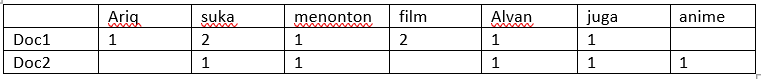
\includegraphics[width=8cm]{figures/1174084/4/teori5.png}
    \centering
    \caption{contoh bag of words}
\end{figure}

\item Jelaskan apa itu TF-IDF.
	\hfill\\
	TF-IDF memberi frekuensi kata dalam setiap dokumen dalam mengganti data jadi number. Ini adalah rasio berapa kali kata itu muncul dalam dokumen dibandingkan dengan jumlah total kata dalam dokumen. Itu meningkat sejalan dengan jumlah kemunculan kata itu di dalam dokumen meningkat. Setiap dokumen memiliki tf sendiri. rumus TF-IDF :
\end{enumerate}
\begin{figure}[H]
    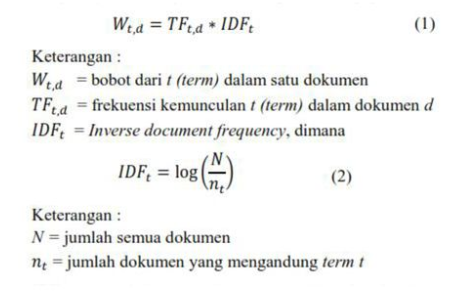
\includegraphics[width=8cm]{figures/1174084/4/teori6.png}
    \centering
    \caption{rumus Tf-IDF}
\end{figure}


\subsection{Praktek}
\begin{enumerate}
\item No. 1
	\hfill\\
	\lstinputlisting[firstline=8, lastline=14]{src/1174084/4/1-2.py}
\begin{figure}[H]
    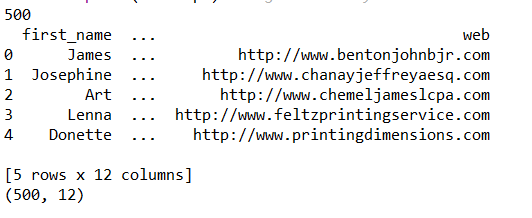
\includegraphics[width=8cm]{figures/1174084/4/1.png}
    \centering
    \caption{aplikasi sederhana pandas}
\end{figure}

\item No. 2
	\hfill\\
	\lstinputlisting[firstline=15, lastline=17]{src/1174084/4/1-2.py}
\begin{figure}[H]
    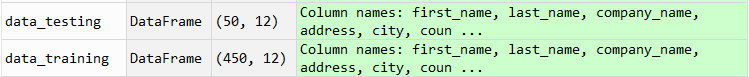
\includegraphics[width=8cm]{figures/1174084/4/2.png}
    \centering
    \caption{pecahan dataframe}
\end{figure}

\item No. 3
	\hfill\\
	\lstinputlisting[firstline=8, lastline=42]{src/1174084/4/3-8.py}
\begin{figure}[H]
    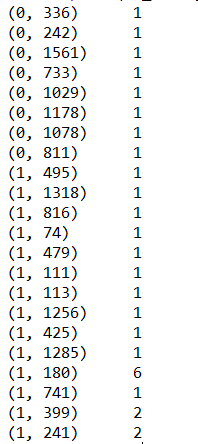
\includegraphics[width=8cm]{figures/1174084/4/3.png}
    \centering
    \caption{vektorisasi dan klasifikasi}
\end{figure}

\item No. 4
	\hfill\\
	\lstinputlisting[firstline=44, lastline=50]{src/1174084/4/3-8.py}
\begin{figure}[H]
    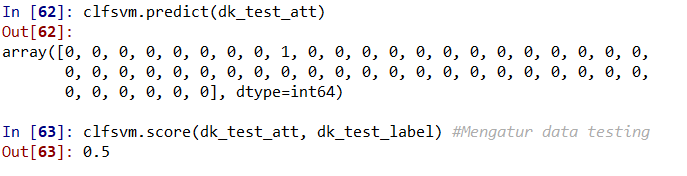
\includegraphics[width=8cm]{figures/1174084/4/4.png}
    \centering
    \caption{klasifikasi SVM}
\end{figure}

\item No. 5
	\hfill\\
	\lstinputlisting[firstline=51, lastline=59]{src/1174084/4/3-8.py}
\begin{figure}[H]
    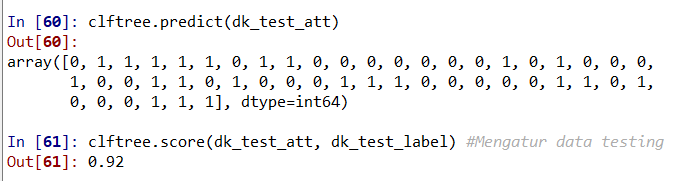
\includegraphics[width=8cm]{figures/1174084/4/5.png}
    \centering
    \caption{klasifikasi Decission Tree}
\end{figure}

\item No. 6
	\hfill\\
	\lstinputlisting[firstline=67, lastline=71]{src/1174084/4/3-8.py}
\begin{figure}[H]
    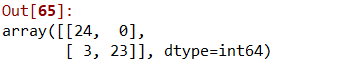
\includegraphics[width=12cm]{figures/1174084/4/6.png}
    \centering
    \caption{confusion matrix}
\end{figure}

\item No. 7
	\hfill\\
	\lstinputlisting[firstline=73, lastline=79]{src/1174084/4/3-8.py}
\begin{figure}[H]
    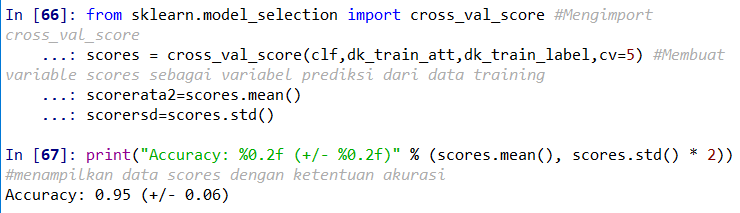
\includegraphics[width=8cm]{figures/1174084/4/7.png}
    \centering
    \caption{cross validaiton}
\end{figure}

\item No. 8
	\hfill\\
	\lstinputlisting[firstline=80, lastline=113]{src/1174084/4/3-8.py}
\begin{figure}[H]
    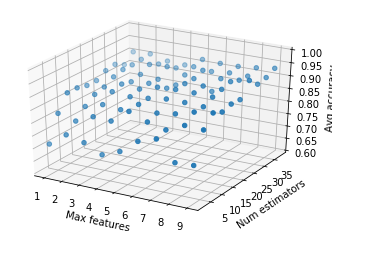
\includegraphics[width=8cm]{figures/1174084/4/8.png}
    \centering
    \caption{pengamatan komponen informasi}
\end{figure}
\end{enumerate}

\subsection{Penanganan Error}
\begin{enumerate}
\item Error
\begin{figure}[H]
    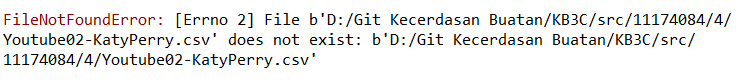
\includegraphics[width=8cm]{figures/1174084/4/error1.png}
    \centering
    \caption{File Not Found Error}
\end{figure}
\item Tuliskan Kode Error dan Jenis Error
	\begin{itemize}
		\item FileNotFoundError
	\end{itemize}
	\item Cara Penangan Error
	\begin{itemize}
		\item FileNotFoundError
		\hfill\break
		Error terdapat pada kesalahan saat baca file csv, yang tidak terbaca. Dikarenakan letak file yang dibaca tidak pada direktori yang sama. Seharusnya letakkan file di direktori yang sama. 
	\end{itemize}
\end{enumerate}

\subsection{Bukti Tidak Plagiat}
\begin{figure}[H]
	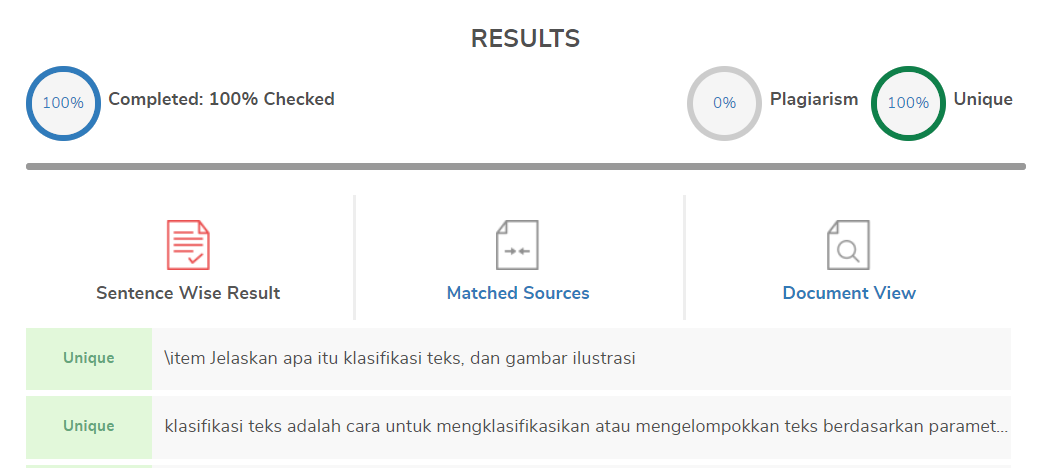
\includegraphics[width=4cm]{figures/1174084/4/plagiarism.png}
	\centering
	\caption{plagiarism}
\end{figure}


\subsection{Link Video Youtube}
https://youtu.be/v63ayQTw\_MI
